\documentclass[notes]{beamer}


\usepackage{pgfpages}
%\setbeameroption{show notes}
%\setbeameroption{show notes on second screen=right}
\mode<presentation> {
  \usetheme{Warsaw}
  % ou autre ...

  \setbeamercovered{transparent}
  % ou autre chose (il est également possible de supprimer cette ligne)
}

\usepackage[backend=bibtex]{biblatex}
\addbibresource{example.bib} % The filename of the bibliography
\usepackage[french]{babel}
\usepackage[latin1]{inputenc}
\usepackage{times}
\usepackage[T1]{fontenc}
\usepackage{tikz}
\usepackage[export]{adjustbox} %For aligining images left/right
\pgfdeclareimage[height=0.5cm]{le-logo}{logo_ujm}
\logo{\pgfuseimage{le-logo}}
\setbeamertemplate{footline}[frame number]
\usepackage{algorithm} % 2 packages to write pseudocode
\usepackage[noend]{algpseudocode}


%%%%%%%%%%%%%%%%%%%%%%%%%%%
\title[Patterns for SoS Reconfiguration] 
{Automatic Sychronisation of Subtitle Track With Live Audio}
%\subtitle {ne compléter que si l'article possède un sous-titre}

\author[Joshua Fenech] 
%{F.~Petitdemange\inst{1} \and I.~Borne\inst{1} \and J.~Buisson\inst{2}}
{Joshua Fenech}

\institute[]
{
	MLDM\\
	Universit\'e de Jean Monnet\\
	Saint-\'Etienne, France
  %\inst{1}
  %IRISA\\
  %University of South Brittany\\
  %Vannes, France
  %\and
  %\inst{2}%
  %RISA\\
  %Military Academy of St-Cyr\\
  %Vannes, France
}

\date[SESOS 2015] 
{M1 Masters Thesis 2018}



\begin{document}


\begin{frame}
  \titlepage
\end{frame}


\section{Introduction}

\subsection{Introduction}

%---------------------------------------------------------------------------------------------------------------------

\begin{frame}{Problem Motivation}
\begin{figure}
	\centering
	\begin{minipage}{0.45\textwidth}
		\centering
		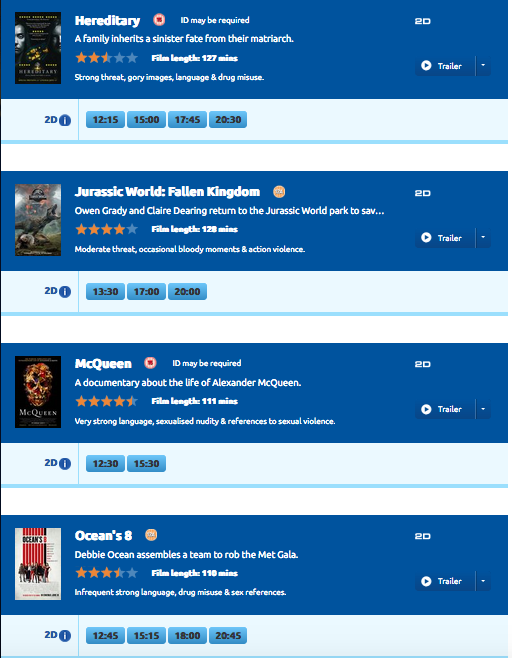
\includegraphics[width=0.9\textwidth]{figures/ALLMOVIESLONDONFULL} % first figure itself
		\caption{Full FIlm Showings 1 Day}
	\end{minipage}\hfill
	\begin{minipage}{0.45\textwidth}
		\centering
		%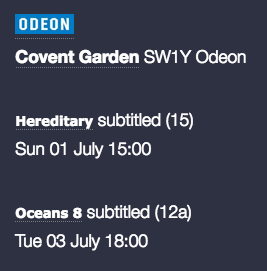
\includegraphics[width=0.9\textwidth]{figures/SUBSMOVIESLONDON} % second figure itself
		%\caption{second figure}
	\end{minipage}
\end{figure}
\end{frame}

%---------------------------------------------------------------------------------------------------------------------

\begin{frame}{Problem Motivation}
\begin{figure}
	\centering
	\begin{minipage}{0.45\textwidth}
		\centering
		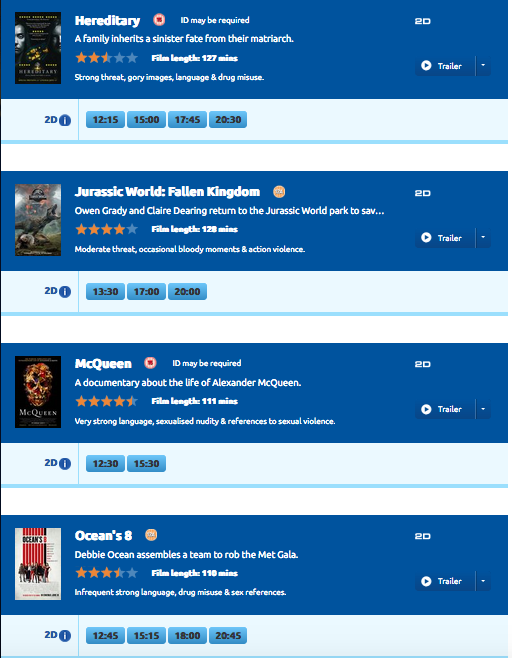
\includegraphics[width=0.9\textwidth]{figures/ALLMOVIESLONDONFULL} % first figure itself
		\caption{Full Film Showings 1 Day}
	\end{minipage}\hfill
	\begin{minipage}{0.45\textwidth}
		\centering
		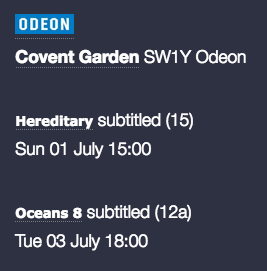
\includegraphics[width=0.9\textwidth]{figures/SUBSMOVIESLONDON} % second figure itself
		\caption{Subtitled FIlm Showings 1 Week}
	\end{minipage}
\end{figure}
\end{frame}

\note{
	\item Number of deaf people
	\item Deaf people feeling excluded
	\item Tourists
	}

%---------------------------------------------------------------------------------------------------------------------

\begin{frame}{Aim}
\begin{itemize}
	\item Develop a method to watch subtitles on a phone
	\item Problem: Synchronising the subtitles to the film
	\item Therefore, must identify the time in the film based on audio signals
\end{itemize}
\end{frame}

%---------------------------------------------------------------------------------------------------------------------

\begin{frame}{Prior Knowledge}
\begin{figure}
	\centering
	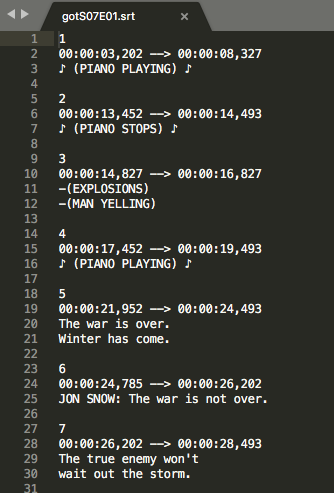
\includegraphics[width=0.35\textwidth]{figures/srt}
	\caption{SubRip .srt File}
\end{figure}
\end{frame}

\note{
	\item Who here has pirated a film?
	\item Used subtitles?
	\item srt
	\item Subrip files contain list of entries indicating start time, stop time and text to be displayed
}

%---------------------------------------------------------------------------------------------------------------------

\begin{frame}{General Method}
\begin{itemize}
	\item Record audio, compressed using MP3
	\item Split signal into frames of duration 25ms - consider signal constant over this period
	\item Take frames every 10ms, so frames overlap
	\item Extract Mel Frequency Cepstral Coefficients (MFCC's) from each frame
	\item Use MFCC's as predictive feature of whether speech is present in a frame or not
	\item Match these predictions to the truth array, defined by a srt file
\end{itemize}
\end{frame}
%---------------------------------------------------------------------------------------------------------------------


\begin{frame}{Prior Knowledge}
\begin{itemize}
  \item How do you use subtitles on a laptop?
  \item SubRip Subtitle file (.srt)
\end{itemize}
\end{frame}


%---------------------------------------------------------------------------------------------------------------------
\section{Preprocessing}
\subsection{Audio Features}
\begin{frame}{MP3 Compression}
\begin{minipage}{0.45\textwidth}
	\centering
	\begin{figure}
		\centering
		\includegraphics[width=\textwidth]{"figures/Frequency Response from Perceptual Coding of Digital Audio NOCAPTION"}
		\caption{Frequency response of human hearing \cite{Painter2000}. Curve indicates amplitude required to detect tone at a given frequency.}
	\end{figure}
\end{minipage}\hfill
\begin{minipage}{0.45\textwidth}
	\begin{figure}
		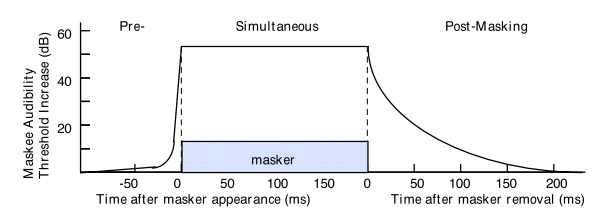
\includegraphics[width=1.2\textwidth]{figures/masking}
		\caption{Frequencies masked by more prevalent frequencies\cite{Painter2000}.}
	\end{figure}
\end{minipage}\hfill
\end{frame}

\subsection{Probability array}
\begin{itemize}
	\item Create array of length appropriate to video with each entry corresponding to a frame
	\item Compare entries of srt to these start/stop times and ascribe a 1 if subtitles are present
\end{itemize}

\begin{algorithm}
	\caption{pb\_array\_fill}\label{euclid}
	\begin{algorithmic}[1]
		\Procedure{}{}
		\State $i \gets 0$
		\State $j \gets 0$
		\State $m \gets pb\_array\_length$
		\State $n \gets subs\_array\_length$
		\While {True}
		%\Procedure{Check arrays not exceeded}
		\If {$i > m$ }  
			\BREAK
			\EndIf
		\If {$j > n$ }  
			\BREAK
			\EndIf
		\If {\textit{pb\_array[i] start time} $\geq$ \textit{subs[j] start time}} 
			\If  {\textit{pb\_array[i] end time} $<$ \textit{subs[j] end time}}
		%\COMMENT {Within subs entry}
				\State $pb\_array[i] \gets 1$
				\State $i \gets i+1$
				\EndIf
		\Else
			\State $j \gets j+1$
		\EndIf
		\EndIf
		\EndProcedure
	\end{algorithmic}
\end{algorithm}
%---------------------------------------------------------------------------------------------------------------------

\begin{frame}{MFCC Audio Features}
\begin{minipage}{0.45\textwidth}
	\centering
	\begin{figure}
		\includegraphics[width=0.9\textwidth]{figures/MFCC_process}
		\caption{Steps of MFCC\cite{mfcc_steps}}
	\end{figure}
	
\end{minipage}\hfill
\begin{minipage}{0.45\textwidth}
\begin{itemize}
	\item Process based on psychoacoustics to represent features most important to human hearing
	\item Split audio file into small sections, consider features constant over this period of time
	\item Apply a series of transformations
	\item Reduce stuff
\end{itemize}
\end{minipage}\hfill
\end{frame}

%---------------------------------------------------------------------------------------------------------------------

\begin{frame}{MFCC Audio Features}

	\centering
	\begin{figure}
		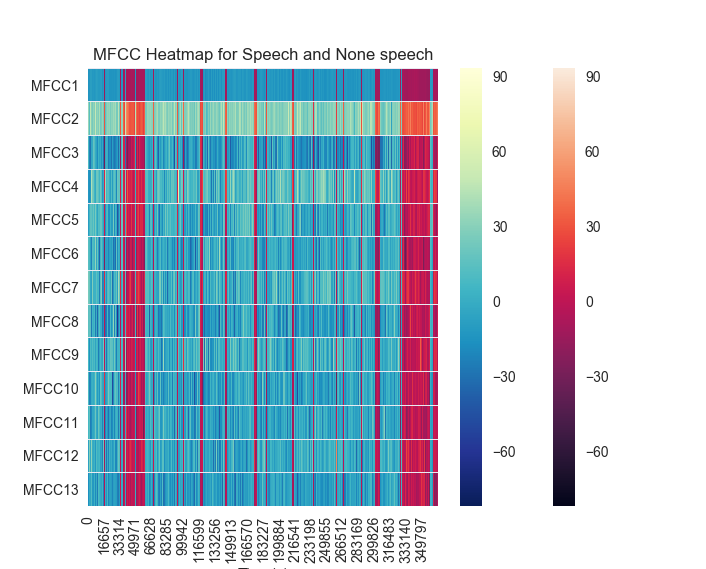
\includegraphics[width=0.7\textwidth]{figures/mfcc_heatmap_speech_or_nospeech}
		\caption{MFCC's Game of Thrones}
	\end{figure}

\end{frame}

%---------------------------------------------------------------------------------------------------------------------

\section{Learner}

\begin{frame}{Learner Architecture}
\begin{minipage}{0.45\textwidth}
	\begin{figure}
		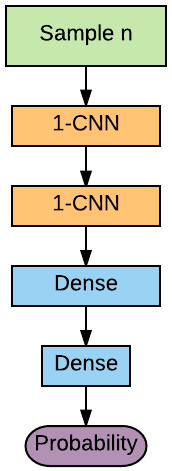
\includegraphics[width=0.4\textwidth]{figures/cnn_sabater}
		\caption{Model architecture\cite{Sabater_2017}}
	\end{figure}
\end{minipage}
\begin{minipage}{0.45\textwidth}
	\begin{figure}
		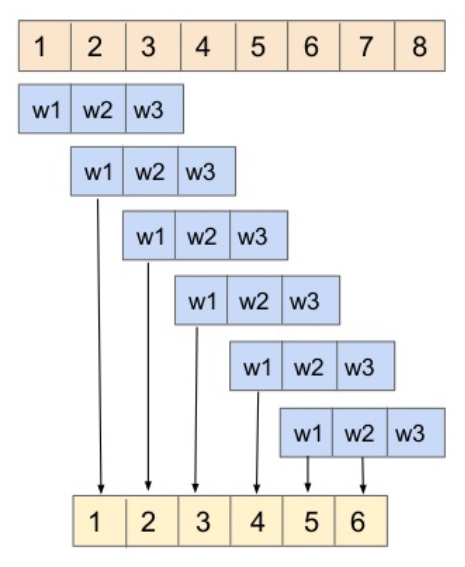
\includegraphics[width=0.7\textwidth]{figures/1dconv_nopad}
		\caption{1d convolutions, no padding \cite{catalunya_2017}}
	\end{figure}
\end{minipage}
\end{frame}

%---------------------------------------------------------------------------------------------------------------------

\subsection{Results}

\begin{frame}{Results}
\begin{figure}
	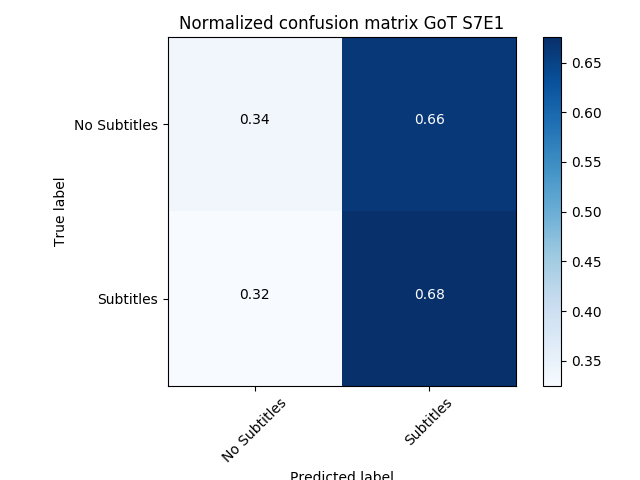
\includegraphics[width=0.7\textwidth]{figures/CM_gots7e1.png}
	\caption{Confusion Matrix Game of Thrones}
\end{figure}
\end{frame}

%---------------------------------------------------------------------------------------------------------------------

\begin{frame}{Results}

\begin{figure}
	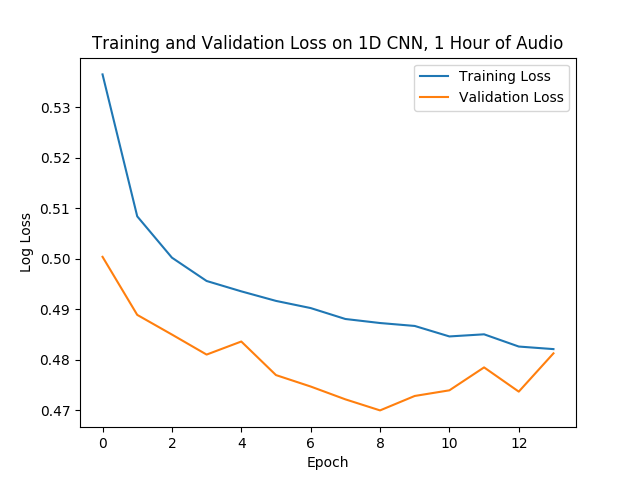
\includegraphics[width=0.7\textwidth]{figures/train_val_loss_run2}
	\caption{Training error}
\end{figure}

\end{frame}
%---------------------------------------------------------------------------------------------------------------------

\begin{frame}{Results}

\begin{figure}
	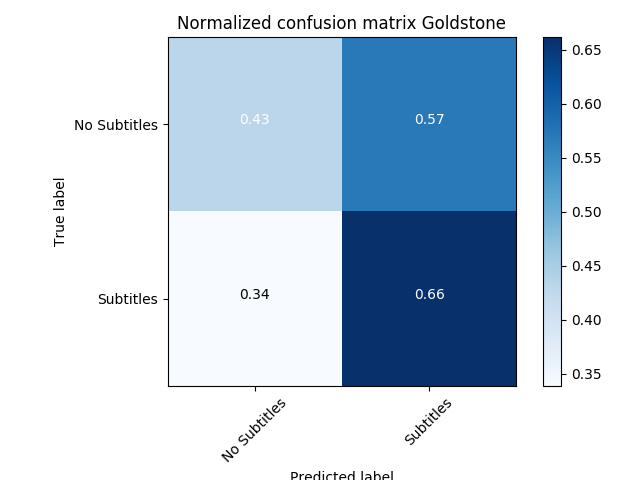
\includegraphics[width=0.7\textwidth]{figures/CM_Goldstone_fixed}
	\caption{Test Time}
\end{figure}

\end{frame}
%---------------------------------------------------------------------------------------------------------------------

\begin{frame}{Results}

\begin{figure}
	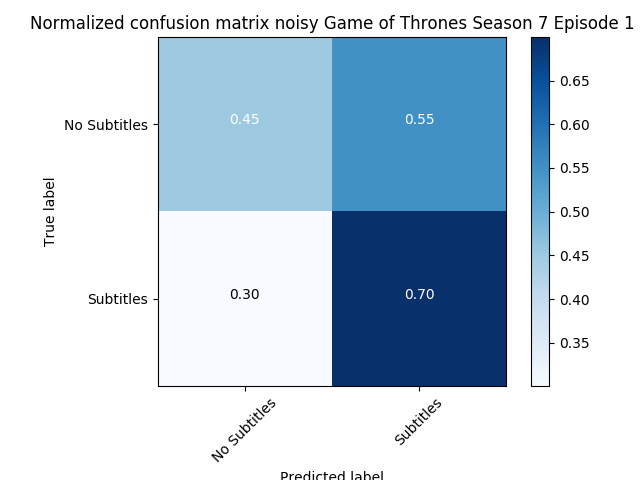
\includegraphics[width=0.7\textwidth]{figures/CM_gots7e1_noisy}
	\caption{Test Time}
\end{figure}

\end{frame}
%---------------------------------------------------------------------------------------------------------------------

\section{Synchronisation}

\begin{frame}{Array Matching}
\begin{figure}
	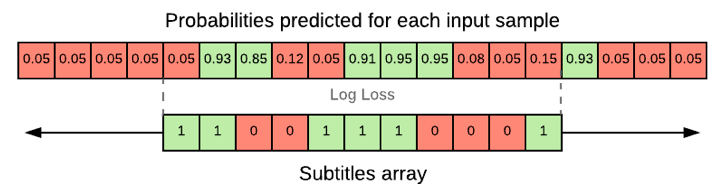
\includegraphics[width=\textwidth]{figures/Array_Matching}
	\caption{Match predictions with truth array using log loss \cite{Sabater_2017}}
\end{figure}
\end{frame}
%---------------------------------------------------------------------------------------------------------------------
\begin{frame}{Synchronisation}
\begin{itemize}
	\item Access to dataset granted incrementally as new audio is recorded
	\item Initially attempted to match a window of predicted probabilities with a similar array generated from srt
	\item Problem: Beginning of film often has no subtitle
	\item Solution: Continue recording data until speech is detected, and identify this as start of subtitle track
\end{itemize}
\end{frame}

%---------------------------------------------------------------------------------------------------------------------
\begin{frame}{Future Work}
\begin{itemize}
	\item Improve accuracy
	\item Remove nonspeech subtitles
	\item More efficient search algorithm
	\item Implement multithreading so that audio can be recorded and features extracted concurrently
	\item Alternative languages
\end{itemize}
\end{frame}

\end{document}